\section{Phuket}

30 mai 2008

\begin{multicols}{2}

Salut tout le monde...

Comment ça je me fais attendre, je vois vraiment pas de quoi vous voulez parler... Mais l'avantage quand les articles sont éspacés dans le temps c'est qu'à priori il va y en avoir plus à lire !! Premièrement j'ai ajouté une video (au début) et 3 photos (à la fin) sur l'article de Langkawi.

Nous voici donc repartis en mer de Langkawi direction Phucket en quelques jours, avec haltes sur différentes îles se trouvant sur notre chemin. But avoué : faire de la plongée car la mer devenait enfin claire. Depuis l'Indonésie impossible de plonger, à certains endroits on voyait à peine le bout de notre bras dans l'eau. Tous ça c'est bien joli, mais c'était compter sans les nuages et la pluie qui rendent la plongée tout de suite moins agréable. Enfin bon on va pas se plaindre quand même.

Nous passons près de Koh Lanta, ça vous dit quelque chose ?

%<div><object width="640" height="505"><param name="movie" value="http://www.dailymotion.com/swf/x5lrzm&related=1"></param><param name="allowFullScreen" value="true"></param><param name="allowScriptAccess" value="always"></param><embed src="http://www.dailymotion.com/swf/x5lrzm&related=1" type="application/x-shockwave-flash" width="640" height="505" allowFullScreen="true" allowScriptAccess="always"></embed></object></div>

Puis nous voici arrivés à Ko Phi Phi, île très touristique, bien que nous soyons en basse saison, le trop plein de monde est blasant. Voici quand même une belle photo, c'est le plus beau coté de la plage principale, l'autre coté étant occupé par des hôtels, restos, boutiques à souvenir...

%\hspace*{-0.65cm}
%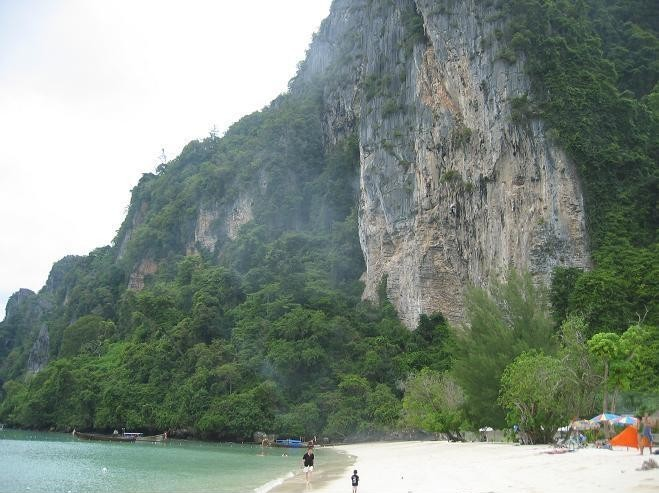
\includegraphics[width=4.8cm]{articles/Phucket/12121623747QwQ.jpg}
%Plage de Ko Phi Phi.

Charlotte, tu reconnais ?

Mais Ko Phi Phi c'est pas pour le tourisme que vous aviez peut être déjà ce nom dans la tête, c'est un des endroits qui a été le plus touché par le tsunami en 2004 et du coup maintenant on se retrouve avec pleins de panneaux de partout indiquant où aller en cas d'alerte.

%\hspace*{-0.65cm}
%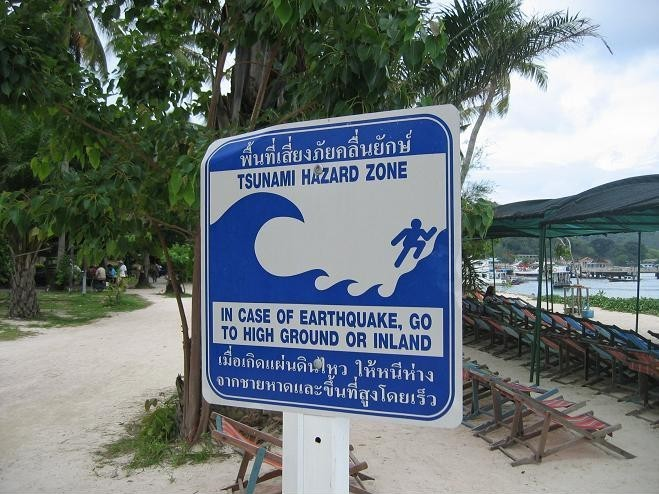
\includegraphics[width=4.8cm]{articles/Phucket/12121623755piH.jpg}
%Panneau d'information suite au tsunami.

Vous remarquerez au passage l'écriture thaï, non non ce n'est pas de la décoration pour faire joli, c'est bien du texte... En plus de ça pour une même orthographe, un mot peut avoir jusqu'à 5 significations différentes suivant sa prononciation. Apprenez le thaï, qu'il disait !!

Ca y est, on arrive à Phuket. Et la, question tourisme, on est en plein dedans : des plages, du béton et... de la prostitution. Phuket Town, la plus grosse ville de l'île échappe un peu à ça, c'est sympa de s'y ballader, on retrouve le quartier chinois, le marché couvert...

%<div><object width="640" height="505"><param name="movie" value="http://www.dailymotion.com/swf/x5lrj3&related=1"></param><param name="allowFullScreen" value="true"></param><param name="allowScriptAccess" value="always"></param><embed src="http://www.dailymotion.com/swf/x5lrj3&related=1" type="application/x-shockwave-flash" width="640" height="505" allowFullScreen="true" allowScriptAccess="always"></embed></object></div>

Sur le reste de l'île, des plages...

%\hspace*{-0.65cm}
%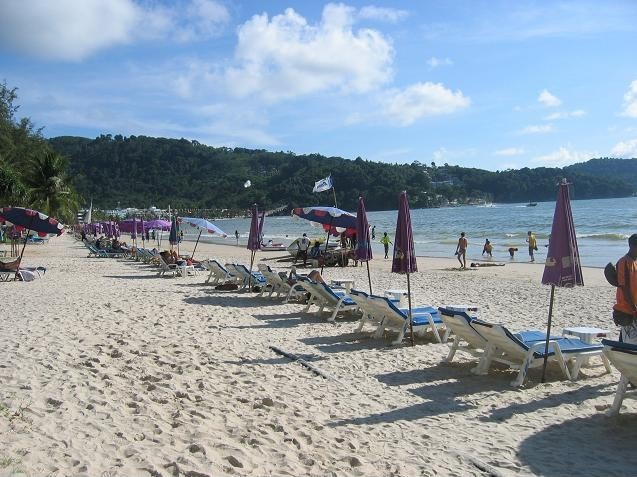
\includegraphics[width=4.8cm]{articles/Phucket/1212162370ANUw.jpg}
%Plage de Phucket.

... et Boat Lagoon, la marina où nous nous sommes arrêtés pour sortir le bateau. En effet Patrick a besoin de faire un carrénage sur le bateau (remettre de la peinture spéciale anti coquillages appelée anti fulling sur la coque) et faire quelques réparations.

%\hspace*{-0.65cm}
%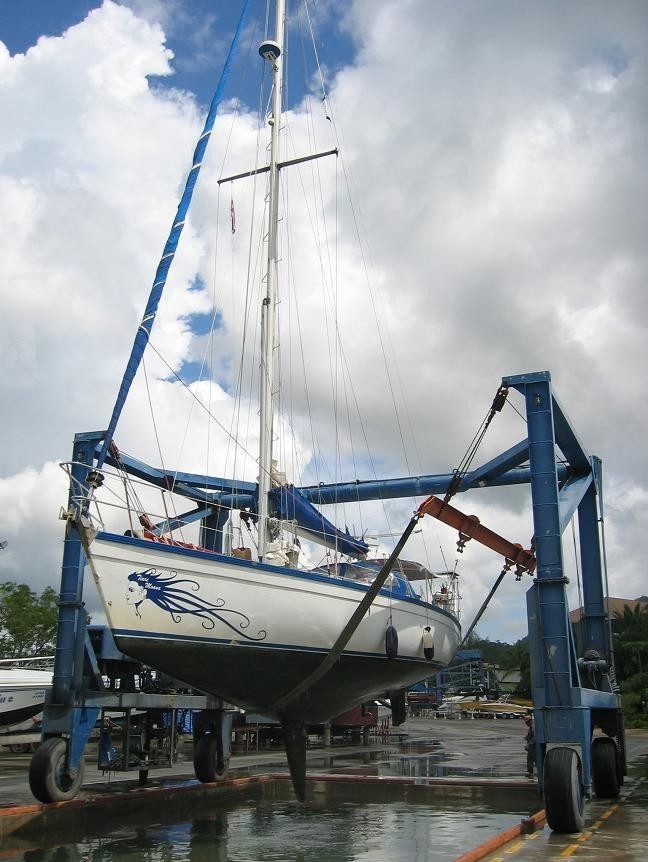
\includegraphics[width=4.8cm]{articles/Phucket/1212162371CgQw.jpg}
%La Tiare Moana sort de l'eau.

%\hspace*{-0.65cm}
%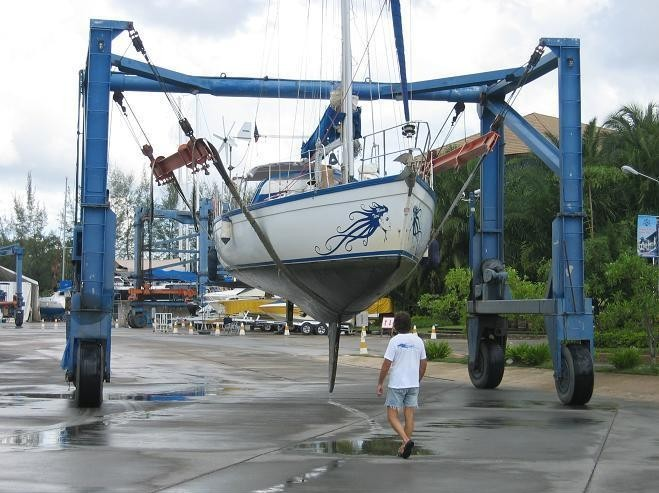
\includegraphics[width=4.8cm]{articles/Phucket/1212162371bVDs.jpg}
%L'est t'y pas bô ce bateau ?

%\hspace*{-0.65cm}
%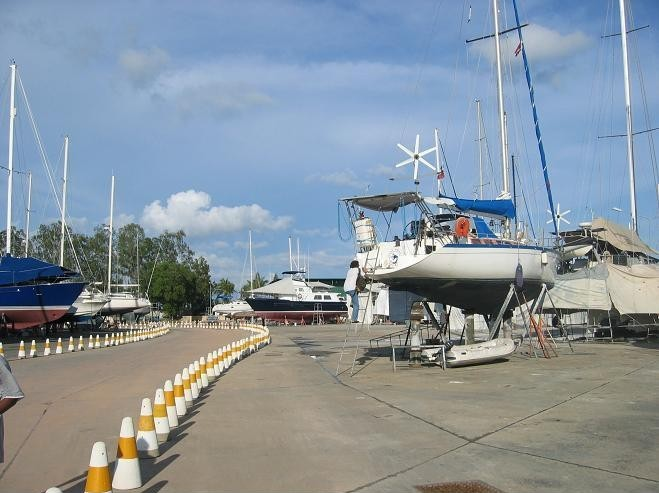
\includegraphics[width=4.8cm]{articles/Phucket/1212162369pBl0.jpg}
%Bon, après, ça fait bizarre de vivre dans un bateau à terre.

Bon... et j'avais pas dit qu'une fois arrivé a Phuket je reprenais mon sac, moi? C'est partiiiiiiii !!!

Jeudi matin, mon sac est fait, je quitte Patrick et son bateau perché à 4 mètres de haut direction Phuket Town. Il faut que j'achète le Lonely Planet car je n'ai pas de guide de la Thaïlande, et que je prenne le bus direction Hua Hin, entre Phuket et Bangkok. Première librairie : pas de guide. Deuxième : les Lonely Planet sont au rayon fiction, ça promet... et ils n'ont pas la Thaïlande, c'est vrai que c'est quand même beaucoup plus utile d'avoir le Brésil ou l'Australie à Phuket. Et puis ils sont aimables comme des portes de prisons, j'arrête, je vais prendre le bus.

Hua Hin please. Je paie, je monte dans le bus, il est 12h30, je n'ai aucune idée du temps de trajet. En premier on me dit 5h, puis 7, puis... j'arrive à 1h du matin après plus de 12 heures de trajet. Je marche un peu, refuse les désormais classiques taxi qui proposent des "cheap hôtel", et zou, je trouve une petite guest house pour dormir, la seule du coin à être ouverte 24h/24 à priori. Bon en même temps je stressais pas trop car Hua Hin est située le long de la mer, et si je ne trouvais rien je serais allé dormir sur la plage, il fait chaud ici y a pas de soucis.

Voila, je crois que je vous ai donné un peu de lecture, à bientôt.

\end{multicols}

\bigskip
\textbf{\textsc{Commentaires}}

\medskip
Titou a écrit le 30 mai 2008 :
\begin{displayquote}
Salut mon ti Dud !
Content d'avoir enfin de tes nouvelles et de voir que ton aventure se poursuit ! Ça y est te revoilà en mode baroudeur solo. Profites à fond et fais bien gaffe à toi.
Continue d'en profiter car ici ce n'est vraiment pas la même chose\dots
Aller gros léchouille et à très bientot !
A plus
\end{displayquote}

\medskip
Cecile a écrit le 04 juin 2008 :
\begin{displayquote}
Ah, les arrivées en ville en pleine nuit après des heures de bus\dots tu dois t'y connaitre maintenant pour dénicher des petits coins sympa ou dormir!
Ca fait plaisir de te voir un p'tit peu sur cette video, t'as l'air en forme tout cas. C'est pas mal d'ailleurs les vidéos, tu fais bien d'en mettre autant que tu peux. On se rend mieux compte d'ici, car bon, les plages paradisiaques ou les buildings super hauts doivent pas forcément être les extraits les plus représentatifs, même si tu nous fait bien baver d'envie avec ça :p
Allez, continue bien ton voyage, courage avec ton sac sur le dos
Gros bisous!
\end{displayquote}

\medskip
Florian a écrit le 08 juin 2008 :
\begin{displayquote}
hello mon ami
je retente de te laisser un message car ca fait deux fois que je tente mais non concluant. tu d'abords je vois que ton voyage se passe bien tu teclate bcp cest cool, tu vois de tres beau paysage. profites en car en france ca fait 10jours qu'il pleut.
pour ma part je ne sais pas encore si je pars qq part cet été, car jai des exam au mois de juillet et si je pars cest vraiment a la derniere minute.
mon ami lui est parti en gouadeloupe pendant 2 mois ils ont loué une maison la bas.
donc je pense ue tu ne dois pas compter sur moi pour faire le vietnam, en tout cas je serai vraiment comtent de te revoir a ton retour en france pour que tu me montre tout ton periple tes photos, que tu nous fasses partager tout ca
je te souhaite bon vent et a la prochaine
\end{displayquote}

\medskip
Etienne a écrit le 10 juin 2008 :
\begin{displayquote}
Salut la compagnie, j'ai un max de retard dans les article mais ca va bientot venir ne vous en faites pas\dots
Je suis passe par Bangkok, puis Kanchanaburi et je suis aujourd'hui a Ayutaya sur la route pour aller a Chiang Mai, vous aurez donc droit a pleins d'infos dans le prochain article, des que j'aurais une bonne connection internet.
Gad, j'ai mis du temps avant de comprendre que c'est toi qui ecrivais\dots pas de Vietnam, tant pis!
Bien le bonjour a tous ceux qui me lisent, et a bientot.
\end{displayquote}

\medskip
Peggy a écrit le 12 juin 2008 :
\begin{displayquote}
kikoo!! je pars quelques jours (en vacances avec des copines, sur des plages moins sensationnelles et beaucoup plus superficielles) et quand je rentre pas de nouvel article!!?
cest quoi cette blague? ahah
allez zou, au boulot !
\end{displayquote}

\medskip
Etienne a écrit le 12 juin 2008 :
\begin{displayquote}
Oui\dots oui\dots
\end{displayquote}

\vfill

